\chapter{Concept}
\label{ch:concept}
This chapter introduces the functional and non-functional requirements of two 
applications - the container runtime and the benchmarking tool. 
In addition, architectural diagrams are provided and discussed. 
Example usage of both applications is shown.
This chapter also contains a thorough justification of the workloads deployed by the benchmarking tool as
well as the variables used to measure the performance of the sandboxed workloads.

\section{Container runtime}
The container runtime is the component responsible for wrapping a user-defined binary 
in a sandbox. It will be used by the benchmarking tool to wrap workloads in sandboxes.

\subsection{Functional requirements}
The Open Containers Initiative standardises the operations \cite{oci-runtime-operations} that 
a container runtime needs to support.

\begin{enumerate}[i]
\item The container runtime must provide clients with state information for a container
given its unique identifier. 
\label{requirements:container-runtime/1}
\item The container runtime must provide clients with the ability to create a new container. 
Users must supply the runtime with a unique identifier for the container and a path to a 
container bundle. The latter consists of a root filesystem and a configuration file that 
defines, amongst other things, the path to the user-defined binary and the set of namespaces
it will reside in.
\label{requirements:container-runtime/2}
\item The container runtime must provide clients with the ability to start a container. 
Users must provide the unique identifier of the container to start. 
This operation must execute the user-defined binary in the sandboxed environment.
\label{requirements:container-runtime/3}
\item The container runtime must allow users to kill the container process.
Users are required to provide the unique identifier of the container and the signal to be sent 
to the container.
\label{requirements:container-runtime/4}
\item The container runtime must allow users to delete the container.
The delete operation must remove all resources allocated in (\ref{requirements:container-runtime/2})
\label{requirements:container-runtime/5}
\item The container runtime must allow external applications to hook into well-defined points 
of a container's lifecycle.
\label{requirements:container-runtime/6}
\end{enumerate}

It is important to note that the container runtime's only responsibility is to sandbox processes. 
An external application, such as the benchmarking tool discussed later, 
must have the ability to interact with the runtime for the purpose of configuring 
the sandboxed environment. This includes operations such as creating network topologies that interconnect 
different containers or allocating shared filesystems. From this, requirement 
(\ref{requirements:container-runtime/6}) has been derived. 

\subsection{Non-functional requirements}
All requirements specified in this section are ranked in order of importance. 
\begin{enumerate}[i]
\item The container runtime must not pollute or damage the host system via its operation.
The runtime manages sensible resources, such as mount points and devices. It must in no way 
cause side effects on the host, leading to operational failure. This is also an important factor 
for allowing reproducibility of the work. Users must be able to use the runtime without fear of 
damaging their system. 
\label{requirements:non-functional/container-runtime/1}
\item The container runtime must support unprivileged containers, i.e containers that run without 
root privileges on the host system. This is in and of itself a functional requirement for running 
containers in multitenant environments. 
\label{requirements:non-functional/container-runtime/2} 
\item The container runtime must be implemented in a programming language with manual memory management.
Satisfying this requirement will ensure that future work aimed at measuring container boot times 
will not be hindered by unpredictable perturbations introduced by a garbage collector.
\label{requirements:non-functional/container-runtime/3}
\item The container runtime must consist of a library component and an executable component. 
This will allow users to implement their own abstractions on top of the library for other research-related 
purposes. 
\end{enumerate}

\subsection{Architecture}
\begin{figure}[H]
    \centering
    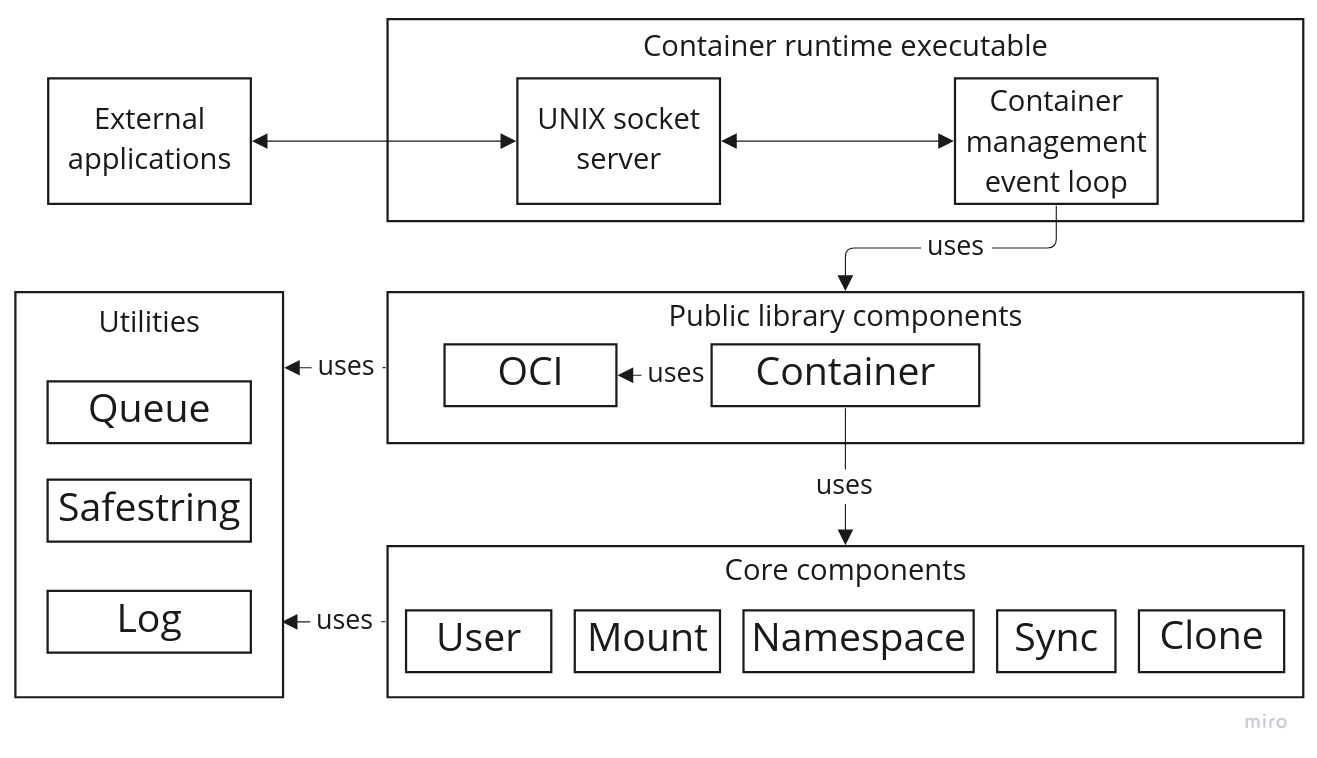
\includegraphics[width=0.55\textwidth]{images/concept/runtime-arch-overview.jpg}
    \caption{High-level overview of the runtime architecture}
    \label{images:concept/runtime-arch-overview.jpg}
\end{figure}
The architecture of the runtime is shown in Figure \ref{images:concept/runtime-arch-overview.jpg}.
It consists of a library and an executable that uses it to provide container 
management services to external applications. The library is split into three parts - utilities,
core components and public components. 

The utilities provide common data structures such as 
linked lists and queues. They also contain procedures for safe string manipulation, a logger,
and a multitude of helper macros that enable the safe management of resources such as file descriptors 
and heap memory. The core components directly interface with the kernel. 
They are responsible for configuring the container, 
i.e the execution environment of the user-defined application. On top, the public library 
components use the core components to provide a 
simple interface for creating, starting, killing and deleting containers. A container 
is represented as an opaque pointer and is only allowed to be accessed through library functions.

The runtime executable uses the container component to create and manage an in-memory queue 
of containers. Furthermore, an additional thread implements an event loop that monitors state changes of all containers 
in the run queue and reaps their resident processes to avoid leaking identifiers.
The main thread of execution implements a UNIX socket server that accepts requests
from external applications, e.g the benchmark tool, to satisfy the functional requirements
defined in the previous paragraph.

\section{Benchmark}

\subsection{Requirements}

\subsection{Methodology}

\subsection{Workloads}

\subsection{User interface}